\documentclass{standalone}
\usepackage{tikz}
\usetikzlibrary{patterns, positioning}
\usepackage[sfdefault]{ClearSans} %% option 'sfdefault' activates Clear Sans as the default text font
\usepackage[T1]{fontenc}

\begin{document}
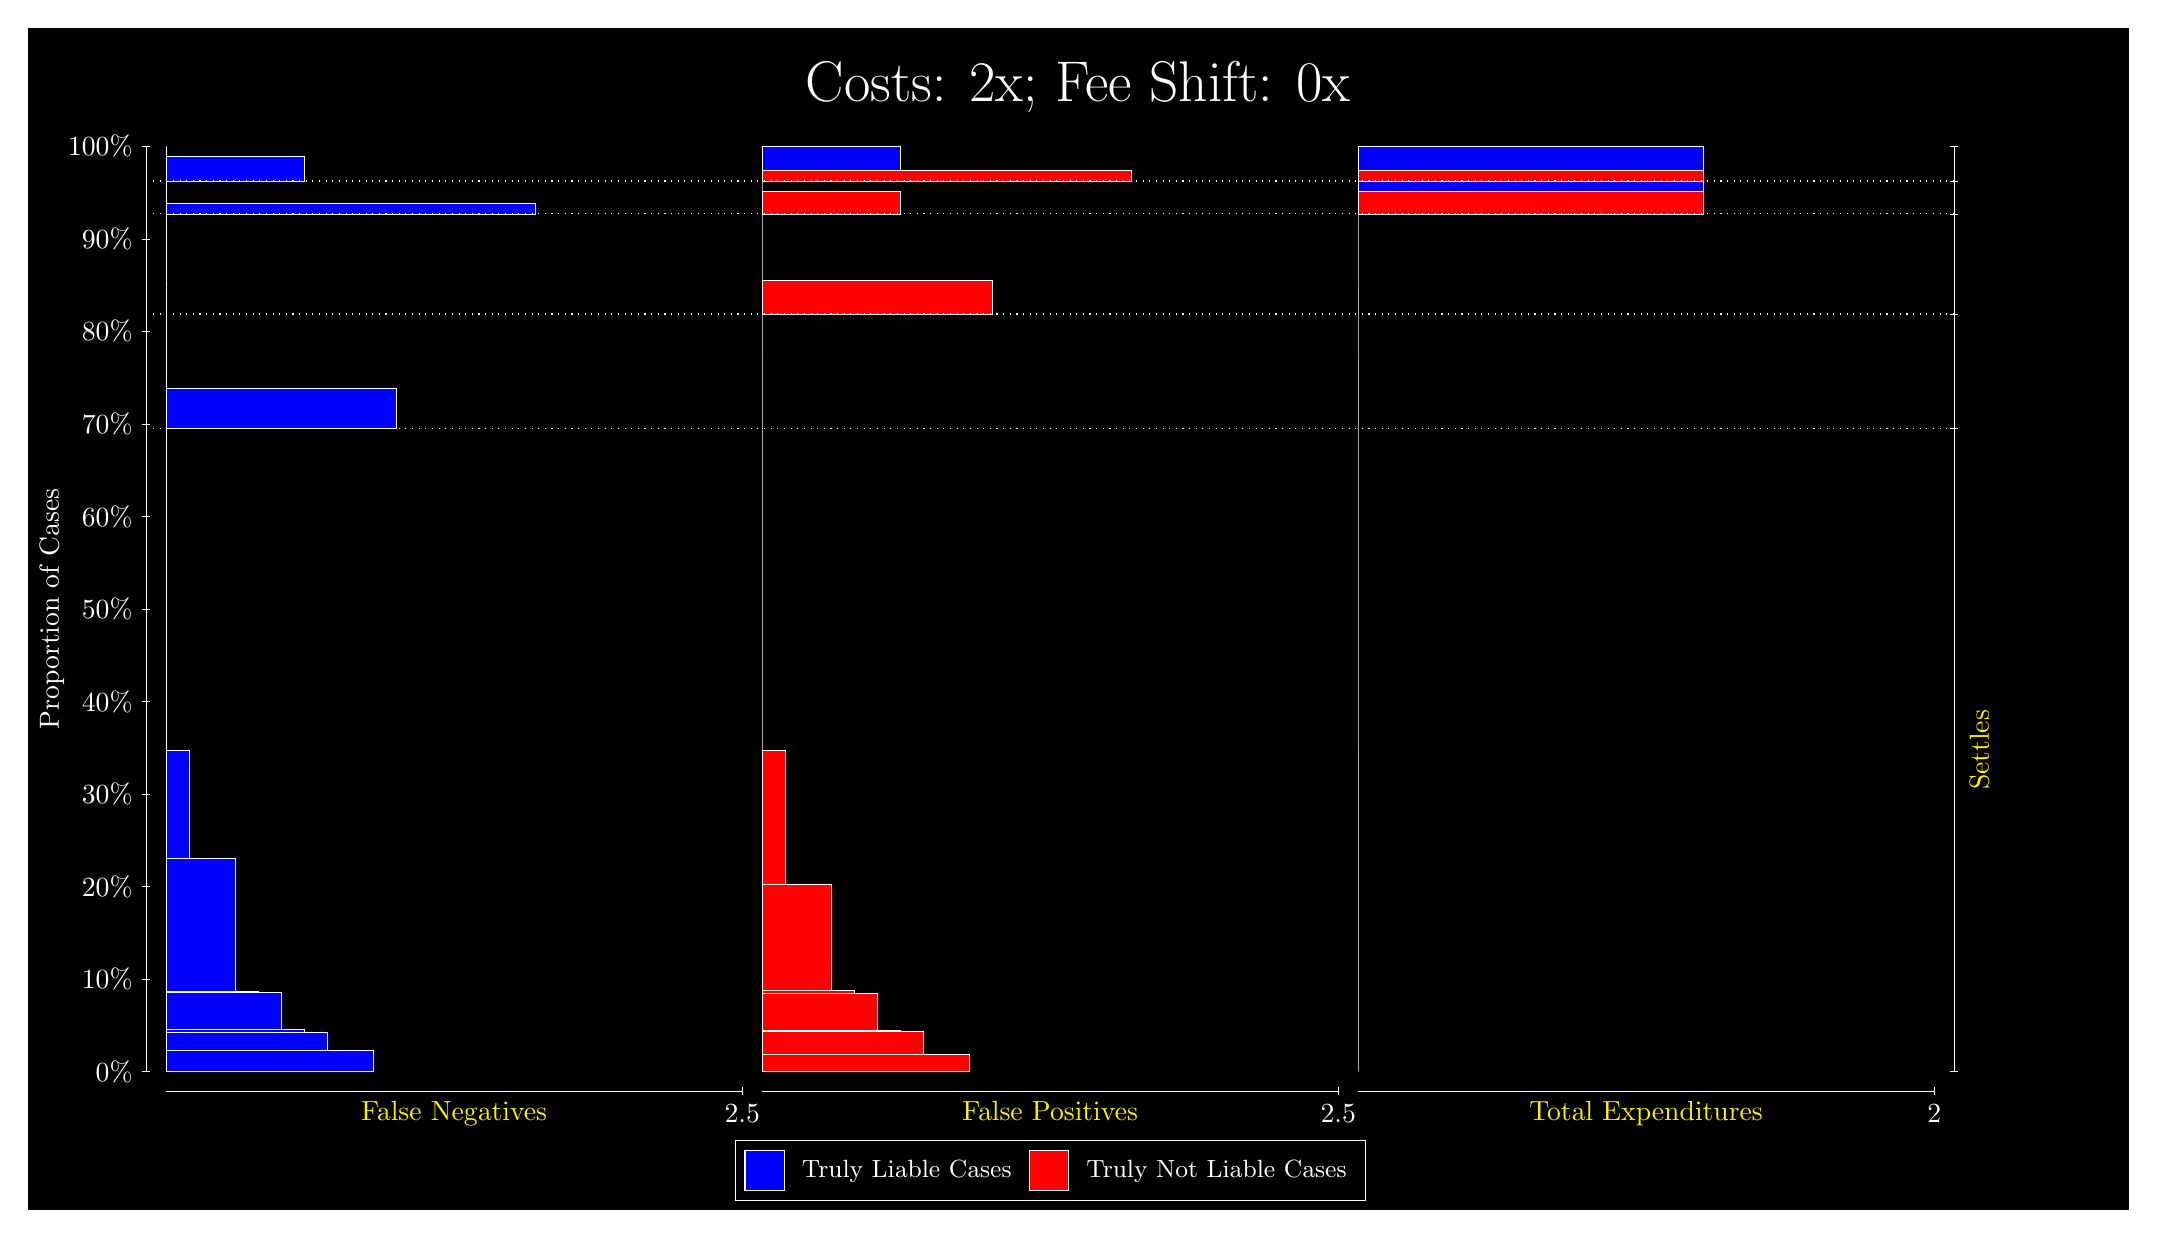
\begin{tikzpicture}
\draw[fill=black] (0,0) rectangle (26.667,15);
\draw[text=white] (0,13.5) rectangle (26.667,15) node[midway] {\huge Costs: 2x; Fee Shift: 0x};
\draw[white, very thin] (1.5,1.75) -- (1.5,13.5);
\node[rotate=90, text=white, anchor=center] at (0.3, 7.625) {Proportion of Cases};
\draw[white, very thin] (1.45,1.75) -- (1.55,1.75);
\node[text=white, anchor=east] at (1.45, 1.75) {0\%};
\draw[white, very thin] (1.45,2.925) -- (1.55,2.925);
\node[text=white, anchor=east] at (1.45, 2.925) {10\%};
\draw[white, very thin] (1.45,4.1) -- (1.55,4.1);
\node[text=white, anchor=east] at (1.45, 4.1) {20\%};
\draw[white, very thin] (1.45,5.275) -- (1.55,5.275);
\node[text=white, anchor=east] at (1.45, 5.275) {30\%};
\draw[white, very thin] (1.45,6.45) -- (1.55,6.45);
\node[text=white, anchor=east] at (1.45, 6.45) {40\%};
\draw[white, very thin] (1.45,7.625) -- (1.55,7.625);
\node[text=white, anchor=east] at (1.45, 7.625) {50\%};
\draw[white, very thin] (1.45,8.8) -- (1.55,8.8);
\node[text=white, anchor=east] at (1.45, 8.8) {60\%};
\draw[white, very thin] (1.45,9.975) -- (1.55,9.975);
\node[text=white, anchor=east] at (1.45, 9.975) {70\%};
\draw[white, very thin] (1.45,11.15) -- (1.55,11.15);
\node[text=white, anchor=east] at (1.45, 11.15) {80\%};
\draw[white, very thin] (1.45,12.325) -- (1.55,12.325);
\node[text=white, anchor=east] at (1.45, 12.325) {90\%};
\draw[white, very thin] (1.45,13.5) -- (1.55,13.5);
\node[text=white, anchor=east] at (1.45, 13.5) {100\%};

\draw[white, very thin] (24.457,1.75) -- (24.457,13.5);
\draw[white, very thin] (24.407,1.75) -- (24.507,1.75);
\node[anchor=west] at (24.407, 1.75) {};
\draw[white, very thin] (24.407,9.9205) -- (24.507,9.9205);
\node[anchor=west] at (24.407, 9.9205) {};
\draw[white, very thin] (24.407,11.37) -- (24.507,11.37);
\node[anchor=west] at (24.407, 11.37) {};
\draw[white, very thin] (24.407,12.643) -- (24.507,12.643);
\node[anchor=west] at (24.407, 12.643) {};
\draw[white, very thin] (24.407,13.059) -- (24.507,13.059);
\node[anchor=west] at (24.407, 13.059) {};
\draw[white, very thin] (24.407,13.5) -- (24.507,13.5);
\node[anchor=west] at (24.407, 13.5) {};

\draw[white, very thin, fill=blue] (1.75,1.75) rectangle (4.3848,2.0185);
\draw[white, very thin, fill=blue] (1.75,2.0185) rectangle (3.7993,2.2516);
\draw[white, very thin, fill=blue] (1.75,2.2516) rectangle (3.5065,2.2915);
\draw[white, very thin, fill=blue] (1.75,2.2915) rectangle (3.2138,2.7538);
\draw[white, very thin, fill=blue] (1.75,2.7538) rectangle (2.921,2.7737);
\draw[white, very thin, fill=blue] (1.75,2.7737) rectangle (2.6283,4.4597);
\draw[white, very thin, fill=blue] (1.75,4.4597) rectangle (2.0428,5.8358);
\draw[white, very thin, fill=red] (1.75,5.8358) rectangle (1.75,9.9205);
\draw[white, very thin, fill=blue] (1.75,9.9205) rectangle (4.6775,10.422);
\draw[white, very thin, fill=red] (1.75,10.422) rectangle (1.75,11.37);
\draw[white, very thin, fill=red] (1.75,11.37) rectangle (1.75,11.796);
\draw[white, very thin, fill=blue] (1.75,11.796) rectangle (1.75,12.643);
\draw[white, very thin, fill=blue] (1.75,12.643) rectangle (6.4341,12.774);
\draw[white, very thin, fill=red] (1.75,12.774) rectangle (1.75,13.059);
\draw[white, very thin, fill=blue] (1.75,13.059) rectangle (3.5065,13.369);
\draw[white, very thin, fill=red] (1.75,13.369) rectangle (1.75,13.5);
\draw[white, very thin, fill=red] (9.3189,1.75) rectangle (11.954,1.9652);
\draw[white, very thin, fill=red] (9.3189,1.9652) rectangle (11.368,2.2554);
\draw[white, very thin, fill=red] (9.3189,2.2554) rectangle (11.075,2.2753);
\draw[white, very thin, fill=red] (9.3189,2.2753) rectangle (10.783,2.74);
\draw[white, very thin, fill=red] (9.3189,2.74) rectangle (10.49,2.7798);
\draw[white, very thin, fill=red] (9.3189,2.7798) rectangle (10.197,4.126);
\draw[white, very thin, fill=red] (9.3189,4.126) rectangle (9.6116,5.8347);
\draw[white, very thin, fill=blue] (9.3189,5.8347) rectangle (9.3189,9.9205);
\draw[white, very thin, fill=red] (9.3189,9.9205) rectangle (9.3189,10.869);
\draw[white, very thin, fill=blue] (9.3189,10.869) rectangle (9.3189,11.37);
\draw[white, very thin, fill=red] (9.3189,11.37) rectangle (12.246,11.796);
\draw[white, very thin, fill=blue] (9.3189,11.796) rectangle (9.3189,12.643);
\draw[white, very thin, fill=red] (9.3189,12.643) rectangle (11.075,12.928);
\draw[white, very thin, fill=blue] (9.3189,12.928) rectangle (9.3189,13.059);
\draw[white, very thin, fill=red] (9.3189,13.059) rectangle (14.003,13.19);
\draw[white, very thin, fill=blue] (9.3189,13.19) rectangle (11.075,13.5);
\draw[white, very thin, fill=red] (16.888,1.75) rectangle (16.888,5.8347);
\draw[white, very thin, fill=blue] (16.888,5.8347) rectangle (16.888,9.9205);
\draw[white, very thin, fill=red] (16.888,9.9205) rectangle (16.888,10.869);
\draw[white, very thin, fill=blue] (16.888,10.869) rectangle (16.888,11.37);
\draw[white, very thin, fill=red] (16.888,11.37) rectangle (16.888,11.796);
\draw[white, very thin, fill=blue] (16.888,11.796) rectangle (16.888,12.643);
\draw[white, very thin, fill=red] (16.888,12.643) rectangle (21.279,12.928);
\draw[white, very thin, fill=blue] (16.888,12.928) rectangle (21.279,13.059);
\draw[white, very thin, fill=red] (16.888,13.059) rectangle (21.279,13.19);
\draw[white, very thin, fill=blue] (16.888,13.19) rectangle (21.279,13.5);
\draw[white, dotted] (1.5,9.9205) -- (24.457,9.9205);
\draw[white, dotted] (1.5,11.37) -- (24.457,11.37);
\draw[white, dotted] (1.5,12.643) -- (24.457,12.643);
\draw[white, dotted] (1.5,13.059) -- (24.457,13.059);
\draw[white, very thin] (1.75,1.5) -- (9.0689,1.5);
\node[text=yellow, anchor=north] at (5.4094, 1.5) {False Negatives};
\draw[white, very thin] (9.0689,1.45) -- (9.0689,1.55);
\node[text=white, anchor=north] at (9.0689, 1.45) {2.5};

\draw[white, very thin] (9.3189,1.5) -- (16.638,1.5);
\node[text=yellow, anchor=north] at (12.978, 1.5) {False Positives};
\draw[white, very thin] (16.638,1.45) -- (16.638,1.55);
\node[text=white, anchor=north] at (16.638, 1.45) {2.5};

\draw[white, very thin] (16.888,1.5) -- (24.207,1.5);
\node[text=yellow, anchor=north] at (20.547, 1.5) {Total Expenditures};
\draw[white, very thin] (24.207,1.45) -- (24.207,1.55);
\node[text=white, anchor=north] at (24.207, 1.45) {2};

\node[text=yellow, centered, rotate=90] at (24.777, 5.8352) {Settles};





\draw (12.978300999999998,1.5) node[draw=none] (baseCoordinate) {};
\begin{scope}[align=center]
        \matrix[scale=0.5, draw=white, below=0.5cm of baseCoordinate, nodes={draw}, column sep=0.1cm]{
            \node[rectangle, draw, minimum width=0.5cm, minimum height=0.5cm, fill=blue] {}; &
            \node[draw=none, font=\small, text=white] (B) {Truly Liable Cases}; &
            \node[rectangle, draw, minimum width=0.5cm, minimum height=0.5cm, fill=red] {}; &
            \node[draw=none, font=\small, text=white] (B) {Truly Not Liable Cases}; \\
            };
\end{scope}

\end{tikzpicture}
\end{document}